% Asset ID: A21TrigonometryAndModellingTikZ-002
% Purpose: Harmonic identity coefficient triangle
\documentclass[tikz,border=10pt]{standalone}
\usepackage{amsmath}
\usetikzlibrary{angles,quotes}
\begin{document}
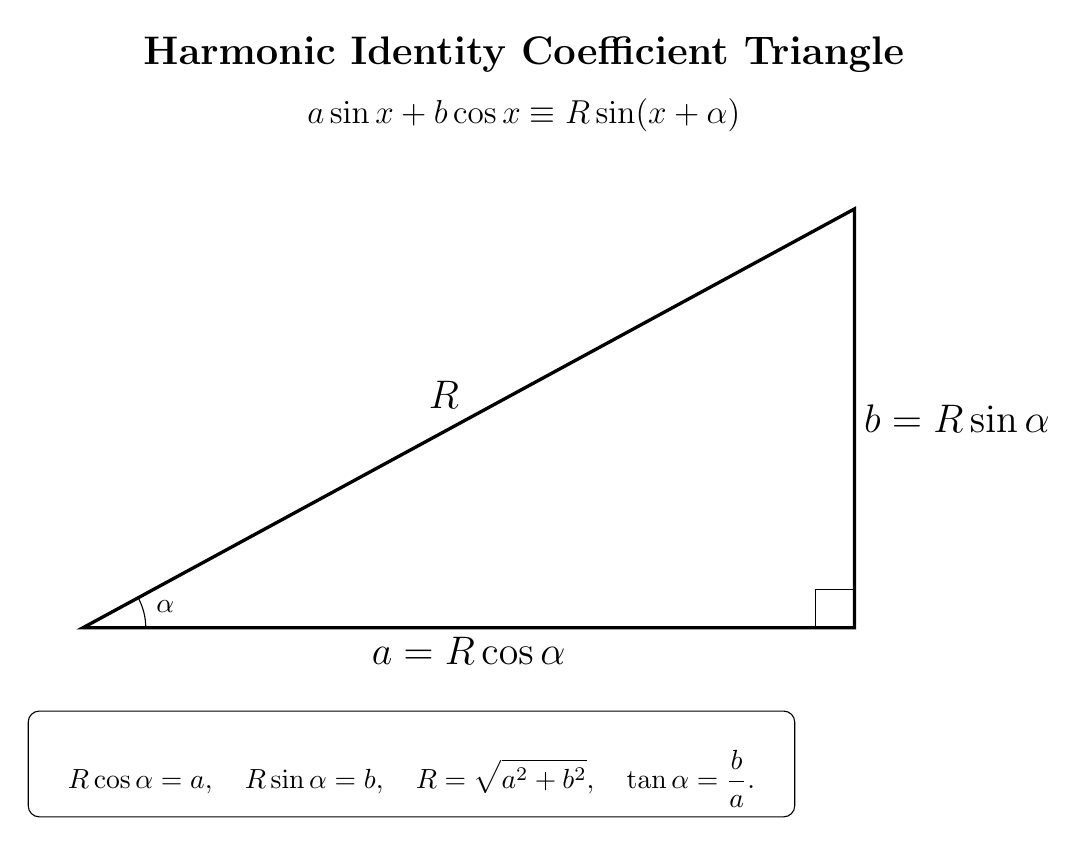
\begin{tikzpicture}[scale=1.4]
\node[font=\Large\bfseries] at (4,5.2) {Harmonic Identity Coefficient Triangle};
\node[font=\large] at (4,4.65) {\(a\sin x+b\cos x\equiv R\sin(x+\alpha)\)};
\coordinate (A) at (0,0); \coordinate (B) at (7,0); \coordinate (C) at (7,3.8);
\draw[very thick] (A)--(B)--(C)--cycle;
\draw (6.65,0) rectangle +(0.35,0.35);
\pic[draw,"$\alpha$",angle radius=0.8cm,angle eccentricity=1.35] {angle=B--A--C};
\node[below] at (3.5,0) {\Large \(a=R\cos\alpha\)};
\node[right] at (7,1.9) {\Large \(b=R\sin\alpha\)};
\node[above left] at (3.5,1.9) {\Large \(R\)};
\node[draw,rounded corners,align=left,text width=9.5cm,anchor=north west] at (-0.5,-0.75)
{\[
R\cos\alpha=a,\quad R\sin\alpha=b,\quad R=\sqrt{a^2+b^2},\quad \tan\alpha=\frac ba.
\]};
\end{tikzpicture}
\end{document}
